\documentclass[11pt,fleqn]{article} 
\usepackage[margin=0.8in, head=0.8in]{geometry} 
\usepackage{amsmath, amssymb, amsthm}
\usepackage{fancyhdr} 
\usepackage{palatino, url, multicol}
\usepackage{graphicx,tabularx,systeme} 
\usepackage[all]{xy}
\usepackage{polynom} 
\usepackage{pdfsync}
\usepackage{enumerate}
\usepackage{framed}
\usepackage{setspace}
\usepackage{array,tikz}

\newcommand{\bbm}{\begin{bmatrix}}
\newcommand{\ebm}{\end{bmatrix}}

\newcommand{\Reals}{\mathbb{R}}
\def\vectwo#1#2{\begin{bmatrix}#1\\#2\end{bmatrix}}
\def\vecthree#1#2#3{\begin{bmatrix}#1\\#2\\#3\end{bmatrix}}
\def\vecfour#1#2#3#4{\begin{bmatrix}#1\\#2\\#3\\#4\end{bmatrix}}

\pagestyle{fancy} 
\lfoot{Linear}
\rfoot{Null Spaces + Geometry}
\renewcommand{\familydefault}{\sfdefault}
\begin{document}

\renewcommand{\headrulewidth}{0pt}
\newcommand{\blank}[1]{\rule{#1}{0.75pt}}
\renewcommand{\d}{\displaystyle}
\vspace*{-0.7in}
\begin{center}
 \textbf{ \large \sc{Null Space and Geometry} }
\end{center}

Return to thinking of the matrix-vector product as a function from $\Reals^n$ to $\Reals^m$ given an $m \times n$ matrix.
\begin{enumerate}
\item Example 1: Let $A=\bbm 1&2\\10&20 \ebm$ and $f(x)=Ax.$\\
	\begin{enumerate}
	\item State $N(A)$. (Recall that we did this on the previous sheet.)
	\vfill
	\item Find the image of the vectors below under $f.$\\
		\begin{enumerate}
		\item $v=(2,-1), \: e_1=(1,0),\: e_2=(0,1)$
		\vfill
		\end{enumerate}
	\item Graph the vectors on the left and their images under $f$ on the right. (Note, I wouldn't chose the same scale on the left as on the right!)
	
	\hspace*{-.3in}
	\begin{tabular}{llr}
	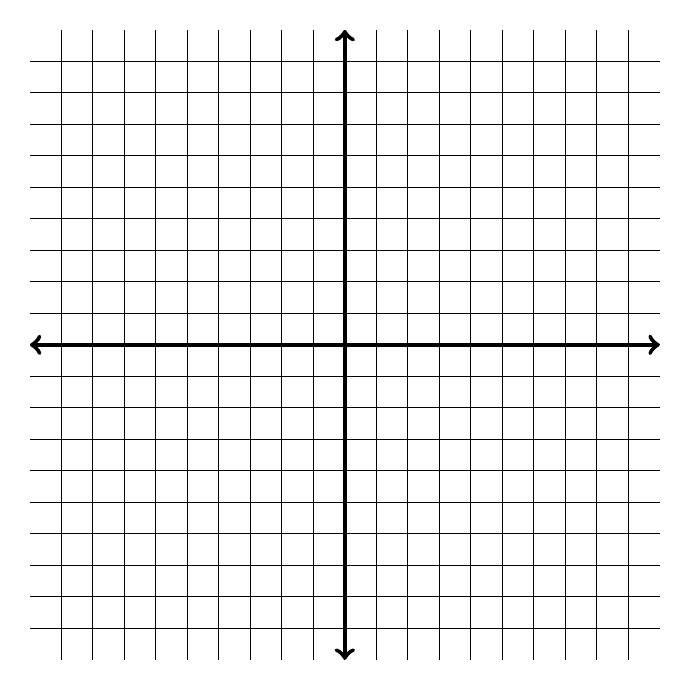
\begin{tikzpicture}[scale=0.4]
	\draw[ultra thick, <->] (-10,0)--(10,0);
	\draw[ultra thick, <->] (0,-10)--(0,10);
	\foreach \i in {-9,-8,...,9}{
		\draw (\i,-10) -- (\i,10);
		\draw (-10,\i) -- (10,\i);
		}
	\end{tikzpicture}
	&
	\quad
	&
	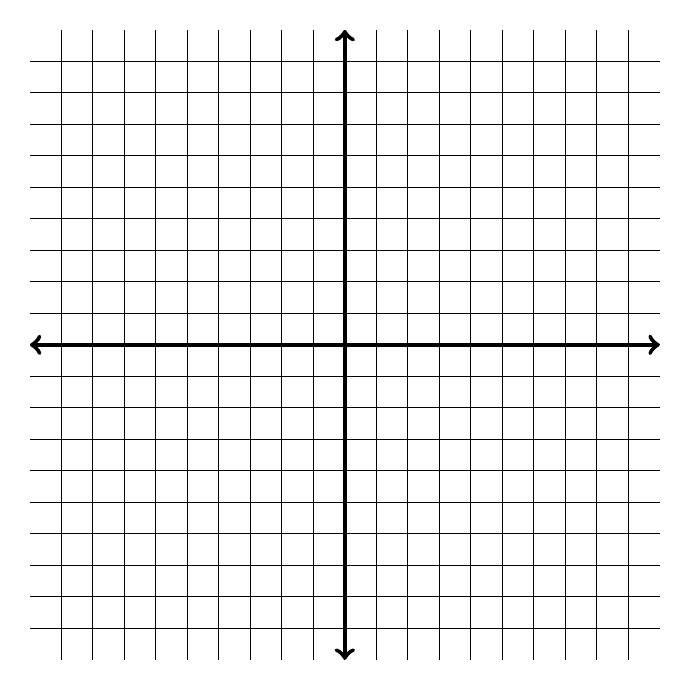
\begin{tikzpicture}[scale=0.4]
	\draw[ultra thick, <->] (-10,0)--(10,0);
	\draw[ultra thick, <->] (0,-10)--(0,10);
	\foreach \i in {-9,-8,...,9}{
		\draw (\i,-10) -- (\i,10);
		\draw (-10,\i) -- (10,\i);
		}
	\end{tikzpicture}
	\end{tabular}
	\end{enumerate}

\vfill
\newpage

\item Example 2: $B=\bbm 2&0\\0&3\ebm$ and $g(x)=Bx.$\\
	\begin{enumerate}
	\item State $N(B)$\\
	\vfill
	\item Find the image of the vectors below under $g.$\\
		\begin{enumerate}
		\item $v=(2,-1), \: e_1=(1,0),\: e_2=(0,1)$
		\vfill
		\end{enumerate}
	\item Graph the vectors on the left and their images under $g$ on the right.
	
	\hspace*{-.3in}
	\begin{tabular}{llr}
	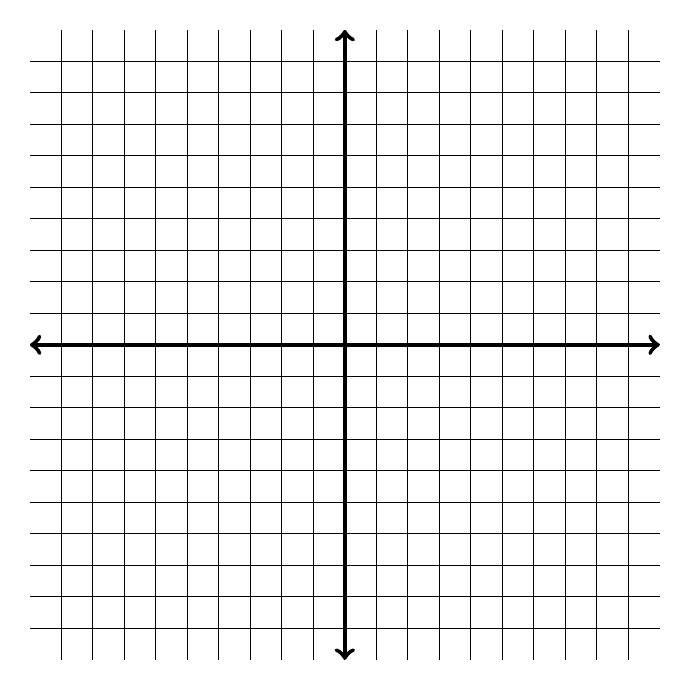
\begin{tikzpicture}[scale=0.4]
	\draw[ultra thick, <->] (-10,0)--(10,0);
	\draw[ultra thick, <->] (0,-10)--(0,10);
	\foreach \i in {-9,-8,...,9}{
		\draw (\i,-10) -- (\i,10);
		\draw (-10,\i) -- (10,\i);
		}
	\end{tikzpicture}
	&
	\quad
	&
	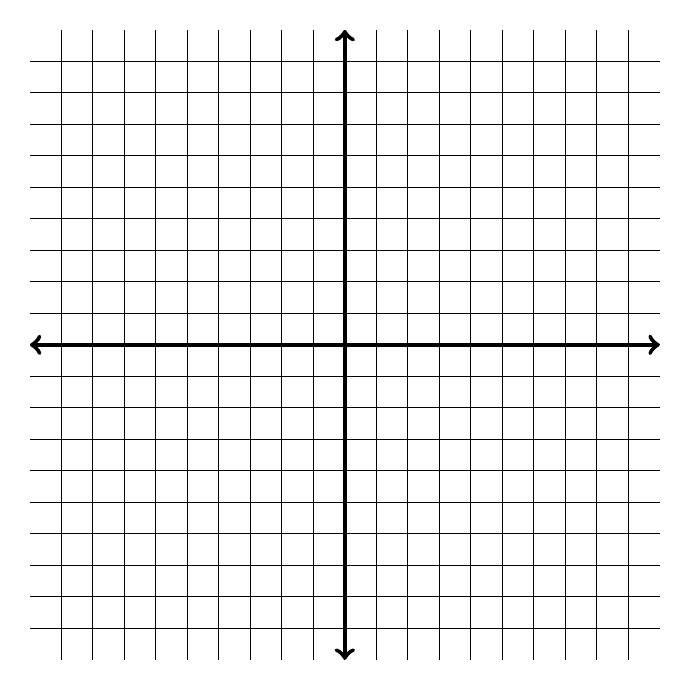
\begin{tikzpicture}[scale=0.4]
	\draw[ultra thick, <->] (-10,0)--(10,0);
	\draw[ultra thick, <->] (0,-10)--(0,10);
	\foreach \i in {-9,-8,...,9}{
		\draw (\i,-10) -- (\i,10);
		\draw (-10,\i) -- (10,\i);
		}
	\end{tikzpicture}
	\end{tabular}
	

	\end{enumerate}

\vfill
\end{enumerate}
\end{document}
	